\documentclass[tikz,border=2pt]{standalone}
\usepackage{amsmath}
\usepackage{mathptmx}
\usetikzlibrary{arrows.meta,automata,positioning}
\definecolor{water}{HTML}{56B4E9}\definecolor{dry}{HTML}{D9C79A}
\begin{document}
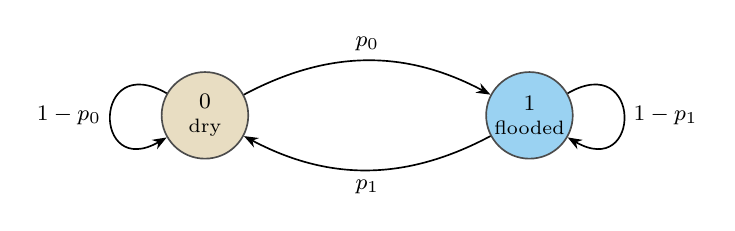
\begin{tikzpicture}[>={Stealth[length=1.8mm]}, font=\footnotesize, node distance=30mm,
  st/.style={circle, draw=black!70, line width=0.6pt, minimum size=11mm, align=center, inner sep=0pt}]
\node[st, fill=dry!60] (d) {$0$\\[-1pt]{\scriptsize dry}};
\node[st, fill=water!60, right=of d] (f) {$1$\\[-1pt]{\scriptsize flooded}};
\draw[->, line width=0.6pt] (d) to[bend left=28] node[above]{$p_0$} (f);
\draw[->, line width=0.6pt] (f) to[bend left=28] node[below]{$p_1$} (d);
\draw[->, line width=0.6pt] (d) to[out=150, in=210, looseness=5] node[left]{$1-p_0$} (d);
\draw[->, line width=0.6pt] (f) to[out=30, in=-30, looseness=5] node[right]{$1-p_1$} (f);
\end{tikzpicture}
\end{document}
